\documentclass[12pt]{article}
\usepackage{geometry}
\geometry{a4paper}
\usepackage[utf8]{inputenc}
\usepackage{amsmath,amssymb}
\usepackage{hyperref} % verlinkungen
\usepackage{textcomp}
\usepackage{flafter}
\usepackage{booktabs}
\usepackage{array}
\usepackage{paralist}
\usepackage{dsfont} \usepackage{color}
\usepackage{bbold}
\usepackage{float}
\usepackage[font=scriptsize,labelfont=bf]{caption}
%\usepackage[font=footnotesize,labelfont=bf]{caption}
\usepackage{subcaption}
\usepackage{fancyhdr}
\setlength{\headheight}{15.2pt}
\pagestyle{fancy}
\usepackage{listings} 
\usepackage{pict2e}
\usepackage{xfrac}
\usepackage[english]{babel}
\usepackage{mathtools}
\usepackage{graphicx}



%%%%%%%%         EIGENEBEFEHLE  %%%%%%%%%
\newcommand{\ddt}{\frac{\partial}{\partial{t}}}
\newcommand{\dnach}[1]{\frac{\partial}{\partial{#1}}}
\newcommand{\ddnach}[2]{\frac{\partial{#1}}{\partial{#2}}}
\newcommand{\dddnach}[3]{\frac{\partial^2{#1}}{\partial{#2} \partial{#3}}}
\newcommand{\dznach}[2]{\frac{\partial^2{#1}}{\partial{#2}^2}}
\newcommand{\vnabla}{\mathbf{\nabla}}
\newcommand{\emathbf}[1]{\mathbf{\hat{#1}}}
\newcommand{\bra}[1]{\langle{#1}|}
\newcommand{\ket}[1]{|{#1}\rangle}
\newcommand{\bracket}[2]{\langle{#1}|{#2}\rangle}
\newcommand{\up}{\uparrow}
\newcommand{\down}{\downarrow}
\newcommand{\updown}{\uparrow\downarrow}
\newcommand{\downup}{\downarrow\uparrow}
\newcommand{\upup}{\uparrow\uparrow}
\newcommand{\downdown}{\downarrow\downarrow}
\newcommand{\sandwich}[2]{\bra{#1} #2 \ket{#1}}
\newcommand{\fsqrt}[2]{\sqrt{\frac{#1}{#2}}}
\newcommand{\GammaK}{{\Gamma_k}}

\definecolor{mygreen}{rgb}{0,0.6,0}
\definecolor{mygray}{rgb}{0.5,0.5,0.5}
\definecolor{mymauve}{rgb}{0.58,0,0.82}

\lstset{%
  backgroundcolor=\color{white},   % choose the background color; you must add \usepackage{color} or \usepackage{xcolor}
  basicstyle=\footnotesize,        % the size of the fonts that are used for the code
  breakatwhitespace=false,         % sets if automatic breaks should only happen at whitespace
  breaklines=true,                 % sets automatic line breaking
  captionpos=b,                    % sets the caption-position to bottom
  commentstyle=\color{mygreen},    % comment style
  %deletekeywords={...},            % if you want to delete keywords from the given language
  %escapeinside={\%*}{*)},          % if you want to add LaTeX within your code
  extendedchars=true,              % lets you use non-ASCII characters; for 8-bits encodings only, does not work with UTF-8
  frame=single,                    % adds a frame around the code
  keepspaces=true,                 % keeps spaces in text, useful for keeping indentation of code (possibly needs columns=flexible)
  keywordstyle=\color{blue},       % keyword style
  language=C,                 % the language of the code
  %morekeywords={*,...},            % if you want to add more keywords to the set
  numbers=left,                    % where to put the line-numbers; possible values are (none, left, right)
  numbersep=5pt,                   % how far the line-numbers are from the code
  numberstyle=\tiny\color{mygray}, % the style that is used for the line-numbers
  rulecolor=\color{black},         % if not set, the frame-color may be changed on line-breaks within not-black text (e.g. comments (green here))
  showspaces=false,                % show spaces everywhere adding particular underscores; it overrides 'showstringspaces'
  showstringspaces=false,          % underline spaces within strings only
  showtabs=false,                  % show tabs within strings adding particular underscores
  stepnumber=2,                    % the step between two line-numbers. If it's 1, each line will be numbered
  stringstyle=\color{mymauve},     % string literal style
  tabsize=2,                       % sets default tabsize to 2 spaces
  %title=\lstname                   % show the filename of files included with \lstinputlisting; also try caption instead of title
}

\lhead[\ ]{\ }
\chead[\ ]{\ }
\rhead[\ ]{\ }

\lfoot[\ ]{\ }
\cfoot[\ ]{\ }
\rfoot[\ ]{\ }

%%%%%%%%%%%%%%%%%%%%%%%%%%%%%%%%%%%%%%%%%%%%

\begin{document}
\title{Temperature Measurements in Optical Tweezer Experiments}
\author{Mathias H\"old, BSc.}
\date{2016}
\maketitle
\thispagestyle{empty}
\newpage
\section{Introduction}
%something about computer science in general, optical tweezers and the need to study the
%systems on computers yada yada





\newpage
\section{Motivation}
%introduction of the experiment, the problem and the idea
\section{The experiment}
The starting point of this thesis is an experiment conducted by Gieseler et al \cite{Gieseler2014}. It is an optical tweezer experiment, where the
motion of a glass nanoparticle in a laser trap was used to investigate the fluctuation theorem\cite{Crooks1999}.
\subsection{Experimental setup}
In the experiment, a silica nano particle with a radius of about 75 nm and mass of about $3 \times 10^{-18}$kg is trapped in a laser beam within a
vacuum chamber. The trapping of the silica nano particle (which will be referred to as \textit{glass particle}) is achieved by a gradient force of the
laser beam acting on the particle. The experimental setup is depicted in fig. \ref{fig:setup}.\\
The particle fluctuates within the trap in all three spatial directions. These fluctuations can be approximated
such that they are decoupled, which means that they can be described by a 1-dimensional Langevin equation:
\begin{equation}
    \ddot{x} + \Gamma_0 \dot{x} + \Omega^2_0x = \frac 1 m \left(F_\text{fluct} + F_\text{ext}\right)
\end{equation}
%The experiment is set up as follows: a glass sphere with radius $r \approx 75$ nm and mass $m \approx 3 \times 10^{-18}$ kg is trapped in a laser beam
%in a vacuum chamber. The initial state of the glass particle is prepared by modulation of the laser, such that the oscillation of the glass particle
%is suppressed in every direction. This is done by measuring the oscillation of the particle in every direction (assuming that the oscillation in every
%direction is decoupled) and using this information as feedback for the laser. This experimental setup can be seen in figure \ref{fig:setup}.
\begin{figure}[H]
    \begin{center}
        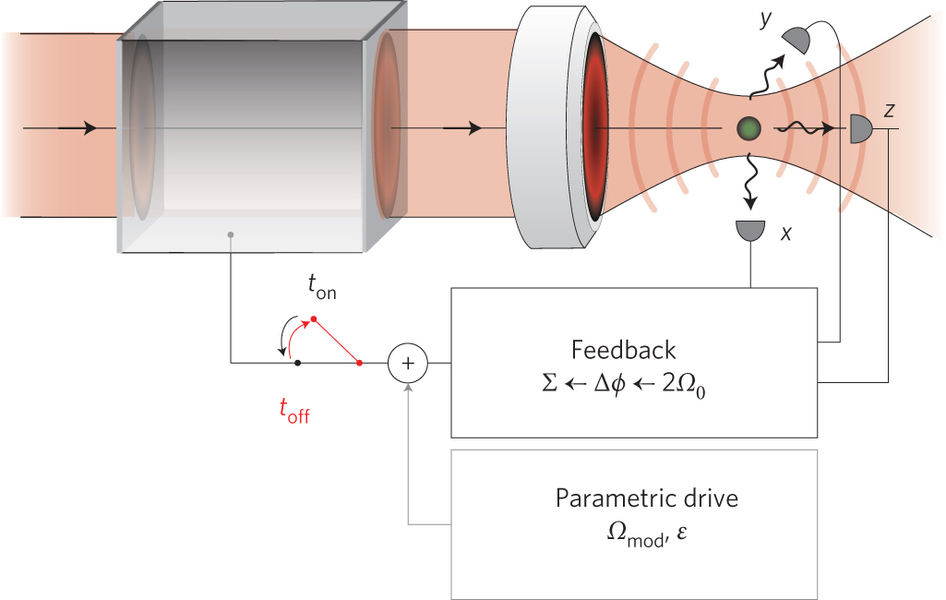
\includegraphics[scale=0.3]{images/experimental_setup.jpg}
        \caption{Experimental setup of the optical tweezer experiment. A silica nano particle is trapped in a laser beam via gradient force in a
        vacuum. The feedback is used to cool down the particle and create a non-equilibrium steady state. In the first part of the experiment, the
    feedback is turned off and the motion of the particle towards an equilibrated state is observed. In the second part of the experiment, the steady state
of the particle is modified by a parametric drive. Both the parametric drive and the feedback are turned off and -- as in the first part -- the
motion of the particle towards an equilibrated state is observerd.}
        \label{fig:setup}
    \end{center}
\end{figure}
On the left hand side we have the friction coefficient $\Gamma_0$ and the angular frequency that describes the fluctuation along the chosen axis. On
the right hand side, there are two forces. The first one is $F_\text{fluct}$, which describes a stochastic force caused by interactions with the gas
in the vacuum chamber. This force is given by
\begin{equation}
    F_\text{fluct} = \sqrt{2m\Gamma_0k_BT_0} \ \xi\left(t\right)
\end{equation}
where $T_0$ is the temperature of the heat bath (i.e. the surrounding gas in the vacuum chamber), $k_B$ is the Boltzmann constant and $\xi(t)$ is
white noise, which obeys the equations $\left\langle\xi(t)\right\rangle= 0$ and $\left\langle\xi(t)\xi(t')\right\rangle= \delta(t-t')$, which means
that it is a random force. The term $\Gamma_0$ appears in the formulat due to the fluctuation-dissipation theorem, which links the damping rate to the
stochastic force.\\
The external force $F_\text{ext}$ is part of the experimental setup, where the frequency of the fluctuation along an axis, $\Omega_0$, is measured and
used to suppress the motion along said axis. This causes a decrease in the particle fluctuations and thus acts as a cooling mechanism for the particle
in the trap. This process creates a non-equilibrium steady state $\rho_{ss}(u,\alpha)$, which is not known analytically. This state is the starting
point of this thesis.\\








\newpage
\section{Simulation}
%simulation techniques and general concept of the simulation itself, used methods and so on 
The problem at hand can be studied on an atomic level with the use of computer simulation. There is a variety of methods for computer simulations
that are widely used, one of which being Molecular Dynamics (MD) simulations. The following section will give a brief overview of the concepts of this
method, which is followed by the application to the simulation of the experiment.

\subsection{Molecular Dynamics}
Molecular Dynamics\cite{Frenkel2001} simulations is a technique for simulating, as the name suggests, the dynamics of a classical many-body system. In this case,
classical means, that the trajectories of the individual particles are calculated using classical mechanics rather then quantum mechanics. For
relatively big atoms/molecules this is a very good approximation, whereas for systems consisting of hydrogen or helium the effects of quantum
mechanics cannot be neglected and other methods (such as ab-initio simulation) has to be used.\\
The dynamics of the system are obtained by solving Newton's equations of motion for every particle. 

\subsection{The Glass Particle}
The glass particle from the experiment will be modeled as a system of particles interacting via a Lennard-Jones pair potential, 
\begin{equation}
    \label{eq:lj}
    U(r) = 4\varepsilon\left[\left(\frac\sigma r\right)^{12} - \left(\frac\sigma r\right)^6\right]
\end{equation}
where $\varepsilon$ is the depth of the potential well (and thus its unit is energy) and $\sigma$ is the distance at which the potential is zero. 
The form of the potential and the relation to the parameters is depicted in Fig. \ref{fig:lj}.
\begin{figure}[h]
    \begin{center}
        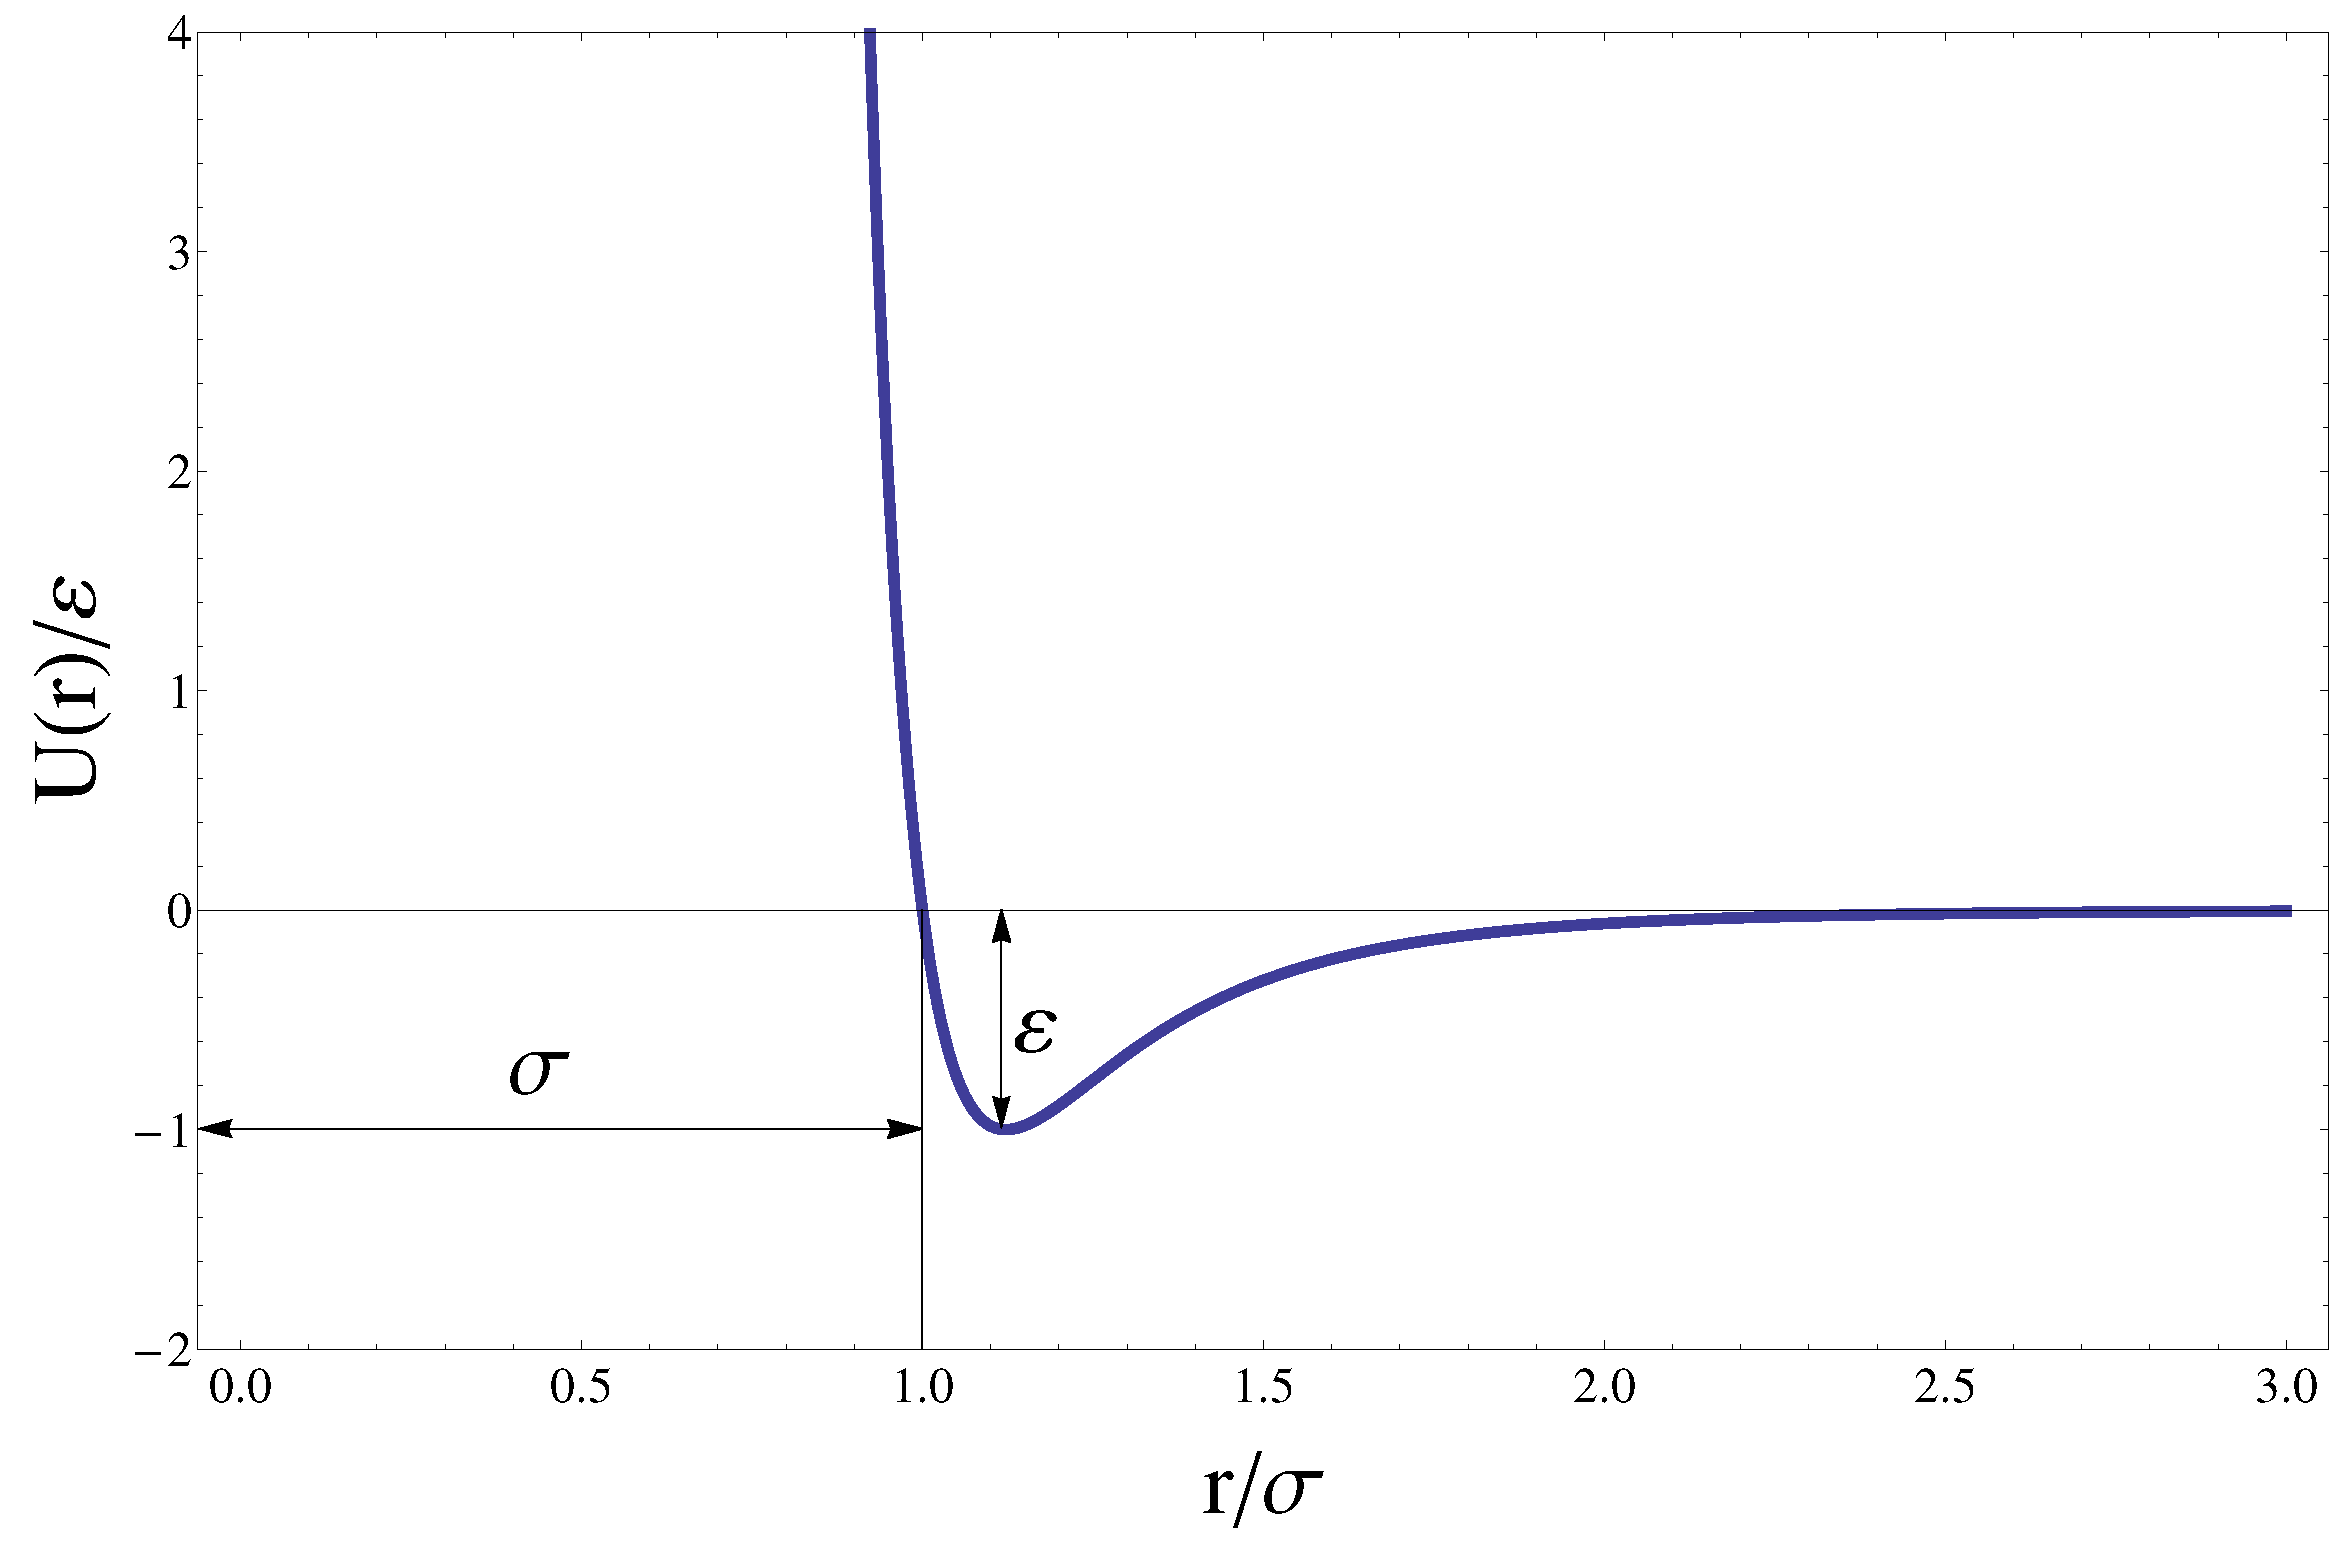
\includegraphics[scale=0.2]{images/LJ-2.pdf}
        \caption{The Lennard-Jones 12-6 potential from \eqref{eq:lj}. The x-axis is the particle distance divided by $\sigma$ and  the y-axis is the
        potential divided by the depth of the potential well.}
        \label{fig:lj}
    \end{center}
\end{figure}
Since $\varepsilon$ and $\sigma$ are crucial parameters for the simulation and do (usually) not change over time, it is practical to use them to
define the dimensions of the system. This means that the unit of distance is $\sigma$, the unit of energy is $\varepsilon$ and the unit of mass is 
the mass of the simulated particle. The so called \textit{reduced units} can be constructed from these three parameters and put into relation to the
original units. Here are some examples:
\begin{itemize}
    \item {distance:} $r^* = r/\sigma$
    \item {potential energy:} $U^* = U/\varepsilon$
    \item {temperature:} $T^* = k_B T/\varepsilon$
    \item {time:} $t^* = t\sqrt{\varepsilon/(m\sigma^2)}$
    \item {pressure:} $P^* = P\sigma^3/\varepsilon$
    \item {density:} $\rho^* = \rho \sigma^3$
\end{itemize}
One very popular choice for the simulated atoms is Argon because it is an inert gas and the atoms behave 
approximately like hard spheres which attract each other with weak van der Waals forces, which justifies the use of the Lennard-Jones potential. 
Argon has a mass of m = $6.69 \times 10^{-26}$ kg, $\sigma = 3.4 \times 10^{-10}$m and $\varepsilon = 1.65 \times 10^{-21}$J.\\
With the above introduced reduced units, the Lennard-Jones potential can be written as
\begin{equation}
    U(r^*) = 4\left[{r^*}^{-12} - {r^*}^{-6}\right].
\end{equation}
Since the reduced units will be used throughout the rest of this thesis, i will drop the asterisk henceforth.\\
From the Lennard-Jones potential the corresponding force can be calculated by taking the derivative with respect to the direction of interest:
\begin{eqnarray}
    F_{x} &=& -\frac{\partial}{\partial x} U(r) \nonumber\\
                &=& -\frac{\partial}{\partial x} 4\left[{r}^{-12} - {r}^{-6}\right] \nonumber\\
                &=& -4 \left[(-12){r}^{-13} - (-6){r}^{-7}\right] \frac{\partial r}{\partial x} \nonumber\\
                &=& 48 \left[r^{-13} - 0.5 \ r^{-7}\right] \frac{x}{r} \nonumber\\
    \label{eq:ljforce} &=& 48 \left[r^{-14} - 0.5 \ r^{-8}\right] x
\end{eqnarray}
The force in the y and z direction can be calculated analogously.\\
The initial configuration of the particles is a face centered cubic (FCC) lattice. A schematic of the FCC lattice is depicted in fig. \ref{fig:fcc}.
With the choice of FCC as initial configuration, there are optimal numbers for the numbers of the particles in the system. Since once FCC cell (as
depicted) shares its atoms with its next neighbours, the number of atom per unit cell is 4, as depicted in fig. \ref{fig:wiki}. The whole system of
atoms is then created by repeating this cell structure. One convenient way is to arrange the unit cells in a cubic system, so if there are $M$ FCC
unit cells on one edge, the whole system consists of $M^3$ cells. Since there are 4 particles per cell, there are ideal or so called \textit{magic
numbers} for atoms for which this setup works perfectly: $N = 4M^3 = 4,32,108,256,500,864,\ldots$.\\
\begin{figure}[h]
    \begin{center}
        \begin{subfigure}[t]{0.3\textwidth}
            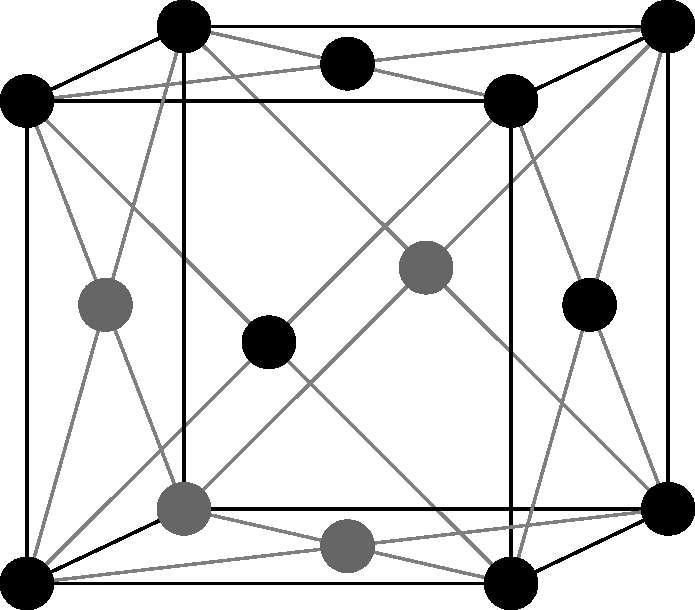
\includegraphics[scale=0.3]{images/fcc-2.pdf}
            \caption{Schematic figure of a face centered cubic (FCC) lattice}
            \label{fig:fcc}
        \end{subfigure} 
        \
        \begin{subfigure}[t]{0.3\textwidth}
            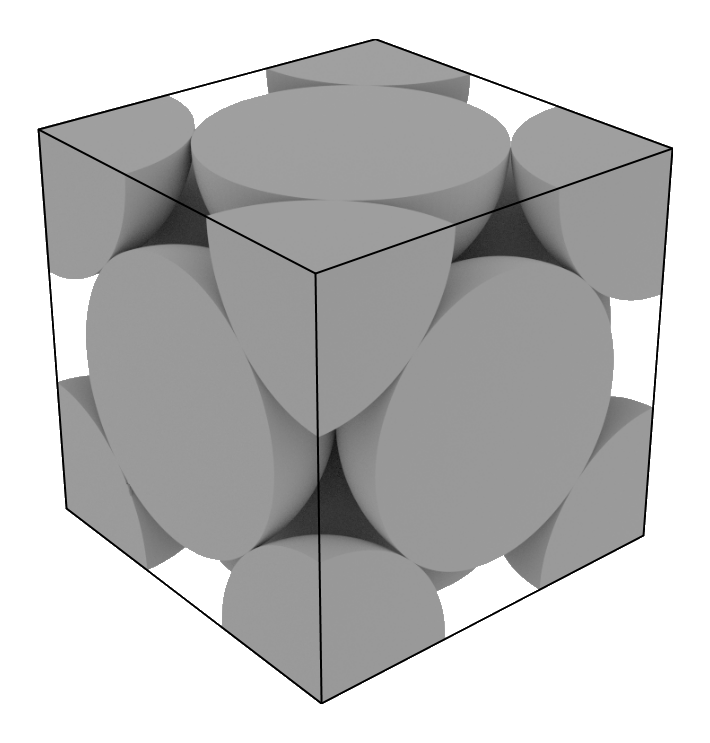
\includegraphics[scale=0.15]{images/fcc_unit.png}
            \caption{Schematic of the number of particles contained in one FCC unit cell. The atoms on the edges are shared by 8 cells and the ones 
                on the faces by 2 cells\cite{unitcell}}
            \label{fig:fcccut}
        \end{subfigure} 
        \
        %\hspace{60pt}
        \begin{subfigure}[t]{0.3\textwidth}
            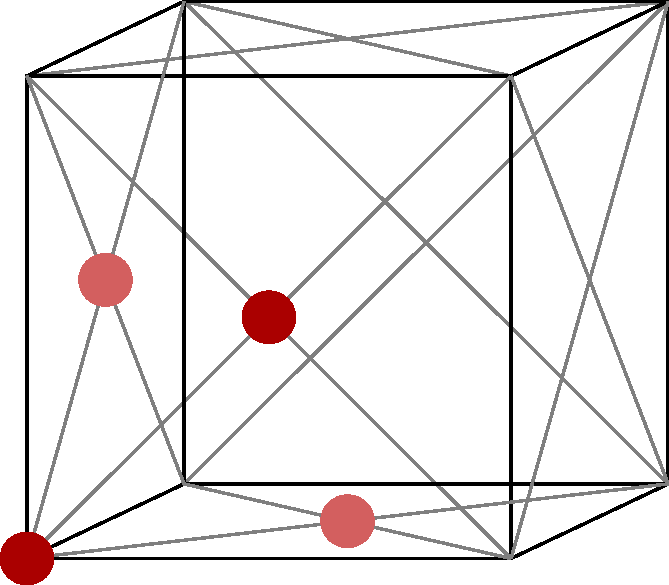
\includegraphics[scale=0.3]{images/unit_cell.pdf}
            \caption{Setup for successively building a FCC lattice}
            \label{fig:unitcell}
        \end{subfigure}
    \end{center}
\end{figure}
%\begin{figure}
    %\begin{center}
        %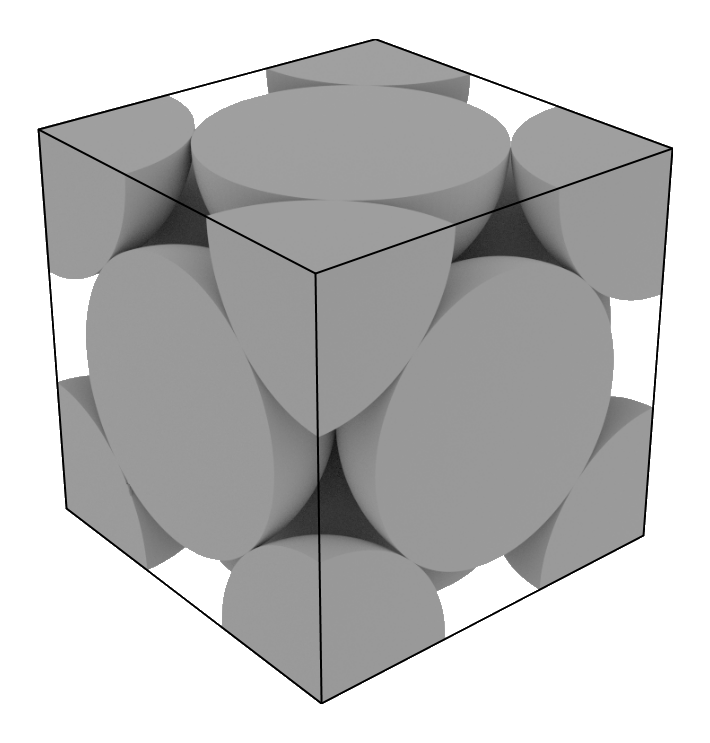
\includegraphics[scale=0.3]{images/fcc_unit.png}
        %\caption{Schematic of the number of particles contained in one FCC unit cell. The atoms on the edges are shared by 8 cells and the ones on the
            %faces by 2 cells. Image taken from
            %{https://upload.wikimedia.org/wikipedia/commons/2/27/Elementarzelle\_einer\_kubisch\_raumzentrierten\_Elementarzelle.png}}
    %\end{center}
%\end{figure}
% do i need to credit the uni buffalo course? 
% http://www.physics.buffalo.edu/phy411-506/
There are several ways to achieve this initial configuration and the one used in this thesis \cite{buffalo} was to create a kind of unit cell 
consisting of four atoms, as shown in fig. \ref{fig:unitcell}, which can be described by a set of points
\begin{eqnarray*}
    p_1 &=& \{0,0,0\}\\
    p_2 &=& \{0.5,0.5,0\}\\
    p_3 &=& \{0.5,0,0.5\}\\
    p_4 &=& \{0,0.5,0.5\}
\end{eqnarray*}
From the particle number $N$ and the number of FCC unit cells per edge $M$ the lattice constant $a$ can be calculated
\begin{equation}
    a = \frac{L}{M}
\end{equation}
where $L$ is the side length of the cube that is the whole system and it is calculated via the density of the system
\begin{equation}
    L = \sqrt[3]{\frac{N}{\rho}}
\end{equation}
With the lattice constant and the 4 points of the FCC cell, all the particles can be put into place.

\subsection{The Velocity-Verlet Algorithm}
When we look at the system from a thermodynamical standpoint, we see that it follows some kind of path in the phase space as time progresses. Every
point in this space corresponds to a set of positions and momenta and the connection between two points corresponds to the evolution of the system
from one state to another. As mentioned above, this evolution (the dynamics of the system) is a crucial element to Molecular Dynamics. Since the
equations of motion cannot be solved analytically in general, we need to approximate the solution.\\
The method used here is called finite difference approach. The trajectory of the system in the phase space is cut into finite pieces of length $\Delta
t$ and the equations of motion are solved for every segment separately (see fig. \ref{fig:finitedifference}).\\
\begin{figure}
    \begin{center}
        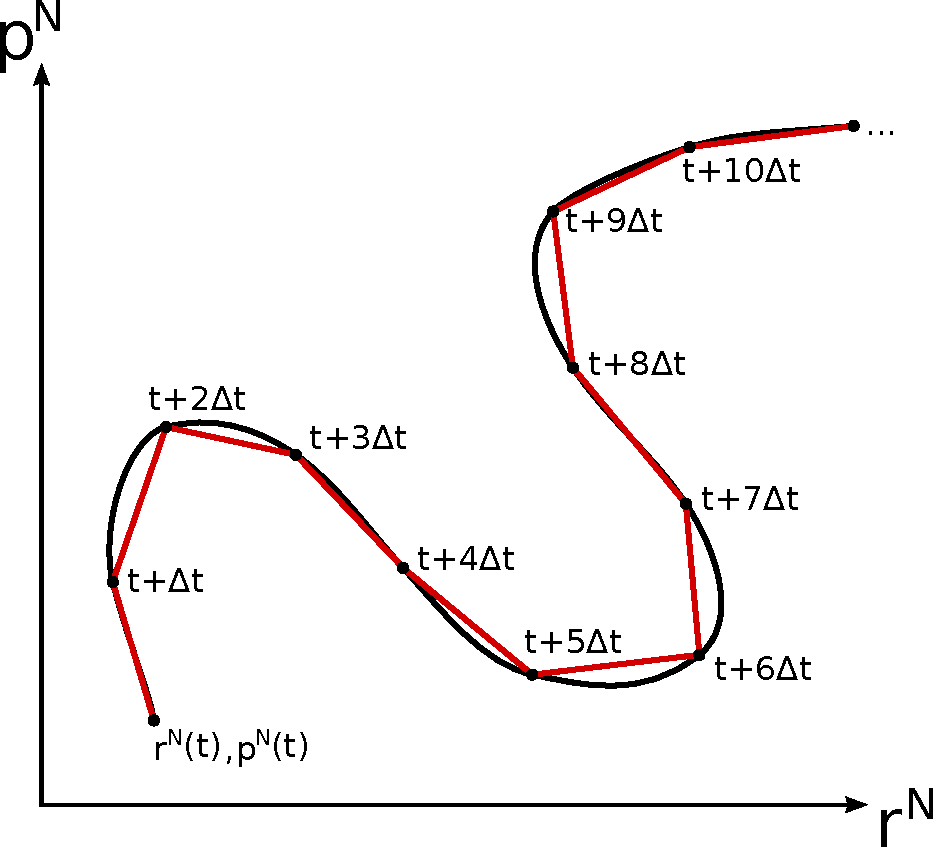
\includegraphics[scale=0.5]{images/finite_approach.pdf}
        \caption{Simplified graphical schematic of the finite difference approach. The evolution of the system from a point $(r^N(t),p^N(t))$ in the
            phase space is approximated by slicing it up into pieces of length $\Delta t$. On every stop after the starting point ($t+\Delta t$, 
            $t+2\Delta t$, $t+3\Delta t$,$\ldots$) the equations of motion can be solved numerically.}
        \label{fig:finitedifference} 
    \end{center}
\end{figure}
There are several ways to solve this kind of problem, but since we are interested in implementing it into a computer program the ideal solution
should have some basic properties \cite{Allen1989}:
\begin{itemize}
    \item It should be fast and require little memory
    \item It should permit the use of a large time step $\Delta t$
    \item It should duplicate the classical trajectory as closely as possible
    \item It should satisfy known conservation laws
    \item It should be simple and easy to program
\end{itemize}
One algorithm that has all of the above mentioned features is the one proposed by Verlet \cite{Verlet1967}. In his paper, Verlet starts by Taylor
expanding the coordinate mathbftor $\mathbf{r}_i$ for one particle after one time step $\Delta t$:
\begin{equation}
    \label{eq:verlet}
    \mathbf{r}_i(t+\Delta t) = \mathbf{r}_i(t) + \dot{\mathbf{r}}_i \Delta t + \frac12 \ddot{\mathbf{r}}_i \Delta t^2 + \frac1{3!} \dddot{\mathbf{r}}_i \Delta t^3 +
    \mathcal{O}(\Delta t^4)
\end{equation}
Since the first derivative of the coordinate mathbftor is the velocity, $\dot{\mathbf{r}}_i(t) = \mathbf{v}_i(t)$, and the second derivative of the coordinate 
mathbftor is the acceleration, $\ddot{\mathbf{r}}_i(t) = \mathbf{a}_i(t)$, using Newton's law $\mathbf{F}_i(t) = m_i \mathbf{a}_i(t)$ equation \eqref{eq:verlet} 
can be written as:
\begin{equation}
    \label{eq:verletnew}
    \mathbf{r}_i(t+\Delta t) = \mathbf{r}_i(t) + {\mathbf{v}}_i(t) \Delta t + \frac1{2m} {\mathbf{F}}_i(t) \Delta t^2 + \frac1{3!} \dddot{\mathbf{r}}_i(t)
    \Delta t^3+\mathcal{O}(\Delta t^4)
\end{equation}
The same calculation can be carried out for one time step before $t$:
\begin{equation}
    \label{eq:verletnewminus}
    \mathbf{r}_i(t-\Delta t) = \mathbf{r}_i(t) - {\mathbf{v}}_i(t) \Delta t + \frac1{2m} {\mathbf{F}}_i(t) \Delta t^2 - \frac1{3!} \dddot{\mathbf{r}}_i(t) \Delta t^3+
    \mathcal{O}(\Delta t^4)
\end{equation}
The sum of those two equations yields
\begin{equation}
    \mathbf{r}_i(t+\Delta t) + \mathbf{r}_i(t-\Delta t) = 2\mathbf{r}_i(t) + \frac1{2} {\mathbf{F}}_i(t) \Delta t^2 + \mathcal{O}(\Delta t^4)
\end{equation}
and from this we get the final form for the new coordinates:
\begin{equation}
    \label{eq:verletfinal}
    \mathbf{r}_i(t+\Delta t) = 2\mathbf{r}_i(t)+ \mathbf{r}_i(t-\Delta t)+ \frac1{2} {\mathbf{F}}_i(t) \Delta t^2
\end{equation}
This means that the new coordinates can be calculated using the current coordinates, the current forces and the coordinates from the past time step.\\
From equation \eqref{eq:verletfinal} one thing becomes clear: the velocities are not necessary to calculate the new positions and they are not
computed in the process, but for the calculation of i.e. the kinetic energy the velocities are needed. Thus, the velocities have to be calculated with
a combination of the Taylor expansions of the coordinate mathbftors at $t+\Delta t$ and $t-\Delta t$:
\begin{equation}
    \mathbf{r}_i(t+\Delta t) - \mathbf{r}_i(t-\Delta t) = 2\mathbf{v}_i(t)\Delta t + \mathcal{O}(\Delta t^3)
\end{equation}
which can be rewritten as
\begin{equation}
    \label{eq:velocities}
    \mathbf{v}_i(t) = \frac{\mathbf{r}_i(t+\Delta t) - \mathbf{r}_i(t-\Delta t)}{2\Delta t} + \mathcal{O}(\Delta t^2)
\end{equation}
This approach has the advantage that it is fast, requires little memory and is reliable in the sense that there is no energy drift occuring during the
simulation, which means that the energy is conserved. When we compare this to the list of desired properties this seems like a good algorithm.\\
This algorithm however has two significant disatvantages. The first one is the calculation of the velocities. As can be seen in equation
\eqref{eq:velocities}, the accuracy of the calculation is only $\mathcal{O}(\Delta t^2)$ while the positions can be calculated with an error of order
$\Delta t^4$. The other big disatvantage is the first step of the algorithm. Since the calculation of the new positions requires the current positions
and the ones from one time step before, which technically do not exist.\\
The solutions to this problem is to include the stepwise calculation of the velocities \cite{swope1982}. For this we start again with the Taylor
expansion of the coordinates mathbftor \eqref{eq:verletnew} and instead of Taylor expanding $\mathbf{r}_i(t-\Delta t)$, we write it as 
\begin{equation}
    \mathbf{r}_i(t) = \mathbf{r}_i(t+\Delta t) - \mathbf{v}_i(t+\Delta t) \Delta t + \frac1{2m} \mathbf{F}_i(t+\Delta t) \Delta t^2
\end{equation}
Using \eqref{eq:verletnew} in the abvove equation we get
\begin{equation}
    \begin{aligned}
        \mathbf{r}_i(t) &= \mathbf{r}_i(t) + \mathbf{v}_i(t) \Delta t + \frac1{2m}\mathbf{F}_i(t)\Delta t^2 \\
                     &- \mathbf{v}_i(t+\Delta t) \Delta t + \frac1{2m} \mathbf{F}_i(t+\Delta t) \Delta t^2
    \end{aligned}
\end{equation}
and thus
\begin{equation}
    \label{eq:vvelocities}
    \mathbf{v}_i(t+\Delta t) = \mathbf{v}_i(t) + \frac1{2m} \left(\mathbf{F}_i(t) + \mathbf{F}_i(t+\Delta t)\right) \Delta t
\end{equation}
With the addition of this equation this algorithm is called the Velocity-Verlet algorithm, which is summarized in the following two equations:
\begin{equation}
    \label{eq:velocityverlet}
    \begin{aligned}
        \mathbf{r}_i(t+\Delta t) = \mathbf{r}_i(t) + {\mathbf{v}}_i(t) \Delta t + \frac1{2m} {\mathbf{F}}_i(t) \Delta t^2\\
        \mathbf{v}_i(t+\Delta t) = \mathbf{v}_i(t) + \frac1{2m} \left(\mathbf{F}_i(t) + \mathbf{F}_i(t+\Delta t)\right) \Delta t
    \end{aligned}
\end{equation}
This algorithm is self starting, uses a small amount of memory, conserves the energy and gives a very good approximation to the originial trajectory
in the phase space. To program this algorithm the following steps are needed: 
\begin{enumerate}
    \item Calculate all the forces between the particles (for the first run only)
    \item Calculate the new positions with current velocity and forces
    \item Calculate first half of the new velocities with current forces
    \item Calculate all the forces for the new position
    \item Use new forces to calculate second half of new velocities
\end{enumerate}
The first point only has to be carried out for the first run, because the forces have not been calculated at this point. As the forces are calculated
for the new positions in step 4, they can be used for the next time step. For the first time step the velocities have to be chosen randomly and are 
calculated with this algorithm from that point forward.

\subsection{The Laser Beam - Energy influx}
The glass sphere is trapped in the laser beam. While the motion of the center of mass is suppressed, which acts as a cooling mechanism, the
individual atoms that make up the glass sphere absorb the energy from the laser which increases their velocity.\\
To simulate this kind behaviour, thermostat algorithms \cite{Huenenberger2005} such as the Nos\'e-Hoover \cite{Nose1984,Hoover1985} or the Berendsen
\cite{Berendsen1984} algorithms.\\
The problem with these kind of algorithms is, that a target temperature has to be fixed which will be reached at some point. In order to simulate the
influx of energy from the laser it would be better to have an algorithm that supplies the system with a certain amount of energy continuously.
Fortunately, such an algorithm exists.\\
The algorithm is called Heat Exchange Algorithm (HEX) \cite{Hafskjold1993}. Its intended purpose is the use in non-equilibrium molecular dynamics
(NEMD) to study transport phenomena and determine transport coefficients. The algorithm works by introducing two regions in the system, one serving as
a heat source and the other as a heat sink. A specific amount of heat is then exchanged between those two reservoirs. As it turns out however, this
algorithm introduces an energy shift for longer simulation times. This led Wirnsberger et al \cite{Wirnsberger2015} to revisit the algorithm and 
identify the cause of this energy drift, to create a more suitable algorithm, which they called eHEX.\\
As in the HEX algorithm, regions are introduced to the system which act either as heat sinks or heat sources. These are labelled with $\Gamma_k$,
where $k > 0$, and have corresponding amount of exchanged heat $\Delta Q_{\Gamma_k}$. If $\Delta Q_{\Gamma_k}$ is negative, heat is subtracted from
the system and vice versa. Regions that neither act as heat source or heat sink are labelled with $\Gamma_0$, which are also called
Hamiltonian regions (see fig. \ref{fig:ehex}). 
\begin{figure}
    \begin{center}
        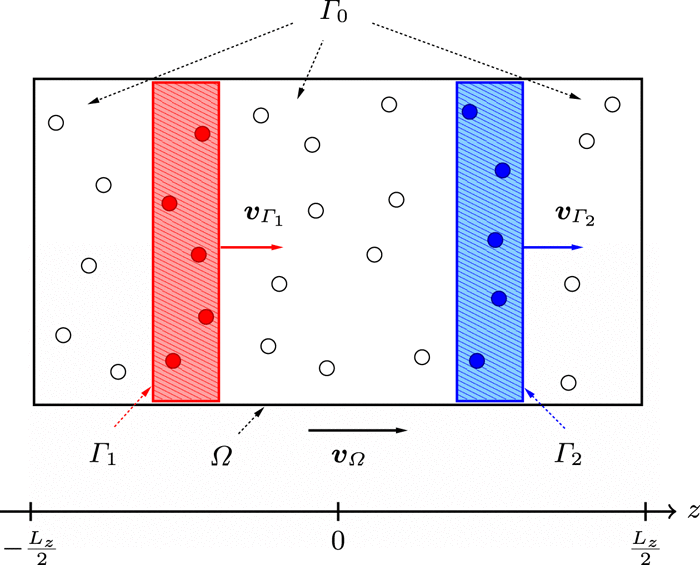
\includegraphics[scale=0.3]{images/ehex_system.png}
        \caption{Setup for the use of the HEX and eHEX algorithms. The simulationbox $\Omega$, which is moving with a velocity of $v_\Omega$,
        contains a heat source (red), $\Gamma_1$, which is moving with velocity $v_{\Gamma_1}$ and a heat sink (blue), $\Gamma_2$, which is moving 
        with velocity $v_{\Gamma_2}$. The regions that are neither heat sources or heat sinks are denoted by $\Gamma_0$.}
        \label{fig:ehex} 
    \end{center}
\end{figure}
The simulation box, denoted by $\Omega$, and the regions $\Gamma_k$ are assumed to be moving with velocities $v_\Omega$ and $v_{\Gamma_k}$
respectively.\\
The change of the energy in a region $\Gamma_k$ is achieved by rescaling the velocities by a factor $\xi_k$ and shifted by the velocity of the
corresponding region:
\begin{equation}
    \mathbf{v}_i \rightarrow \mathbf{\bar{v}}_i = \xi_k \mathbf{v}_i + (1-\xi_k)\mathbf{v}_{\Gamma_k}
\end{equation}
The bar over a quantity denotes the value after the exchange of heat.\\
The factor $\xi_k$ is given by
\begin{equation}
    \xi_k = \sqrt{1+\frac{\Delta Q_{\Gamma_k}}{\mathcal{K}_{\Gamma_k}}}
\end{equation}
where $\Delta Q_{\Gamma_k}$ is the exchanged heat in the region $\Gamma_k$ and $\mathcal{K}_{\Gamma_k}$ is the non-translational kinetic energy of the
region $\Gamma_k$ and is given by
\begin{equation}
    \label{eq:kineticK}
    \mathcal{K}_{\Gamma_k} = \sum_{i \in \gamma_k} \frac{m_i v_i^2}{2} - \frac{m_{\Gamma_k}v_{\Gamma_k}^2}{2}
\end{equation}
The sum is taken over all indices in $\gamma_k$ which is the set of indices of particles in the region $\Gamma_k$.\\
For the final version of the eHEX algorithm there are three more quantities needed. The first one is the heat flux per time step, denoted by 
$\mathcal{F}_\GammaK$:
\begin{equation}
    \mathcal{F}_\GammaK = \frac{\Delta Q_\GammaK}{\Delta t}
\end{equation}
The second one is the thermostatting force $\boldsymbol{\eta}_i$, which is defined as
\begin{equation}
    \boldsymbol{\eta}_i = 
    \begin{cases}
        m_i \ \dfrac{{\mathcal{F}_{\Gamma_{k(\mathbf{r}_i)}}}}{{2\mathcal{K}_{\Gamma_{k(\mathbf{r}_i)}}}} \
        \left(\mathbf{v}_i - \mathbf{v}_{\Gamma_{k(\mathbf{r}_i)}}\right)
        & \quad \text{if } k(\mathbf{r}_i) > 0 \\
        0 & \quad \text{otherwise}
    \end{cases}
    %\begin{cases}
        %m_i \ \frac{\displaystyle{\mathcal{F}_{\Gamma_{k(\mathbf{r}_i)}}}}{\displaystyle{2\mathcal{K}_{\Gamma_{k(\mathbf{r}_i)}}}} \
        %\left(\mathbf{v}_i - \mathbf{v}_{\Gamma_{k(\mathbf{r}_i)}}\right)
        %& \quad \text{if } k(\mathbf{r}_i) > 0 \\
        %0 & \quad \text{otherwise}
    %\end{cases}
\end{equation}
where $k(\mathbf{r}_i)$ is the index of the region in which particle $i$ located, i.e. $k(\mathbf{r}_i) = 0$ means that the particle is in a Hamiltonian
region and $k(\mathbf{r}_i) > 0$ denotes the heat sinks and sources.\\
The last quantity is the one that corrects the long term energy drift of the HEX algorithm, denoted by $\mathcal{E}{r}_{i,\alpha}$.
The analysis and derivation of this term is given in \cite{Wirnsberger2015}.
\begin{equation}
    \label{eq:bigeps}
    \begin{aligned}
        \mathcal{E}{r}_{i,\alpha} &= \dfrac{\eta_{i,\alpha}}{m_i\mathcal{K}_{\Gamma_{k(\mathbf{r}_i)}}} \left[
        \frac{\mathcal{F}_{\Gamma_{k(\mathbf{r}_i)}}}{48} + \frac{1}{6} \sum_{j\in\gamma_{k(\mathbf{r}_i)}} \mathbf{f}_j \cdot \left(\mathbf{v}_j - 
            \mathbf{v}_{\Gamma_{k(\mathbf{r}_i)}}\right)\right] \\
            &- \frac{\mathcal{F}_{\Gamma_{k(\mathbf{r}_i)}}}{12\mathcal{K}_{\Gamma_{k(\mathbf{r}_i)}}} \left[
            \frac{f_{i,\alpha}}{m_i} - \frac{1}{m_{\Gamma_{k(\mathbf{r}_i)}}} \sum_{j\in\gamma_{k(\mathbf{r}_i)}}f_{j,\alpha}\right]
    \end{aligned}
\end{equation}
The $\mathbf{f}$ in the above equation denotes the force corresponding to the chosen intermolecular potential $U(\mathbf{r})$, 
\begin{equation}
    \mathbf{f} = -\nabla_{\mathbf{r}_i} U(\mathbf{r}_i)
\end{equation}
With all the necessary quantities established, the updating sequence of the eHEX algorithm can be written down:
\begin{subequations}
\begin{eqnarray}
    \bar{\mathbf{v}}^n_i &=& \xi^n_{k(\mathbf{r}_i)} \mathbf{v}^n_i + \left(1-\xi^n_{k(\mathbf{r}_i)}\right) \mathbf{v}^n_{\Gamma_{k(\mathbf{r}_i)}} \\
    \bar{\mathbf{v}}^{n+\frac12}_i &=& \bar{\mathbf{v}}^n_i + \frac{\Delta t}{2m_i} \mathbf{f}^n_i\\
    \bar{\mathbf{r}}^{n+1}_i &=& \mathbf{r}^n_i + \Delta t \bar{\mathbf{v}}^{n+\frac12}_i\\
    \mathbf{f}^{n+1}_i &=& \left.-\nabla_{\mathbf{r}_i} U(\mathbf{r})\right|_{\mathbf{r} = \bar{\mathbf{r}}^{n+1}}\\
    \bar{\mathbf{v}}^{n+1}_i &=& \bar{\mathbf{v}}^{n+\frac12}_i + \frac{\Delta t}{2m_i} \mathbf{f}^{n+1}_i\\
    \mathbf{v}^{n+1}_i &=& \bar{\xi}^{n+1}_{k(\bar{\mathbf{r}}_i)} \bar{\mathbf{v}}^{n+1}_i + \left(1-\bar{\xi}^{n+1}_{k(\bar{\mathbf{r}}_i)}\right)
    \bar{\mathbf{v}}^{n+1}_{\Gamma_{k(\bar{\mathbf{r}}_i)}} \\
    \mathbf{r}^{n+1}_i &=& \bar{\mathbf{r}}^{n+1} - \Delta t^3 \mathcal{E}\bar{\mathbf{r}}^{n+1}_i
\end{eqnarray}
\end{subequations}
This algorithm can be applied to the problem of the levitating nano sphere in the laser beam by adjusting the setup and some of the parameters.\\
Firstly, the setup of the heat sinks and sources has to be changed. Since there is only energy pumped into the system from the outside, the region
acting as a heat sink vanishes and the region acting as a heat source spans over the whole simulation box. This means that, using the 
notation of fig. \ref{fig:ehex}, $\Omega = \Gamma_1$. Furthermore, neither the simulation box nor the heat source are moving, i.e. 
$\mathbf{v}_\Omega = \mathbf{v}_{\Gamma_1} = 0$. This affects the non-translational kinetic energy term $\mathcal{K}_{\Gamma_1}$, the thermostatting
force $\boldsymbol{\eta}$ and the correction term $\mathcal{E}\mathbf{r}$. Since there is only one region acting as a heat sink, the terms $\Delta Q$,
$\mathcal{K}$ and $\mathcal{F}$ don't need an index. The summation index in \eqref{eq:kineticK} and \eqref{eq:bigeps} can be changed to the number of
particles in the system, $N$, since all the particles are within the heat exchanging region. The masses are set to 1, i.e. $m_i = 1$ with the chosen
reduced units and with this the total mass of the region (in the term $1/m_{\Gamma_{k(\mathbf{r}_i)}}$ in \eqref{eq:bigeps}) is equal to the number of
particles in the system. With these changes, the quantities can be written down as:
\begin{eqnarray}
    \mathcal{K} &=& \sum_{N} \frac{v_i^2}{2}\\
    \xi &=& \sqrt{1+\frac{\Delta Q}{\mathcal{K}}}\\
    \mathcal{F} &=& \frac{\Delta Q}{\Delta t}\\
    \boldsymbol{\eta}_i &=& 
    \dfrac{\mathcal{F}}{{2\mathcal{K}}} \
        \mathbf{v}_i\\
        \mathcal{E}{r}_{i,\alpha} &=& \dfrac{\eta_{i,\alpha}}{\mathcal{K}} \left[
        \frac{\mathcal{F}}{48} + \frac{1}{6} \sum_{N} \mathbf{f}_j \cdot \mathbf{v}_j
            \right] \nonumber \\
            &-& \frac{\mathcal{F}}{12\mathcal{K}} \left[
            {f_{i,\alpha}} - \frac{1}{N} \sum_{N}f_{j,\alpha}\right]
\end{eqnarray}
This means that the laser is modeled to be pumping energy into the system, which increases the velocities of the velocities of the particles in the
system over time, while the center of mass motion is not affected by this.\\


\subsection{Surrounding Gas - Barostat}
Without any equilibrating mechanism the setup described by now would lead to the system melting, which is not desirable. In the next step we will 
introduce the surrounding gas of the gas chamber that will absorb some of the energy in the system, leading to the final state.\\
Generally, pressure is introduced to the system by surrounding the object of interest (in this case the glass nano sphere) with a pressure medium.
There are two main requirements for the choice of such a pressure medium: the exerted pressure must be hydrostatic and the computation of the
interaction between the pressure medium and the object of interest must not take up a lot of resources.\\
The model used in this thesis was developed by Gr\"unwald and Dellago \cite{Gruenwald2006} and uses an ideal gas of non-interacting particles as
pressure medium. The particles of this pressure medium flow into the simulation from an outside box, whose geometry is based on the form of the object
of interest. This barostat also acts as a thermostat and thus is suitable for the application in this thesis.\\
The gas particles interact with the object via a soft-sphere potential of the form
\begin{equation}
    \label{eq:softsphere}
    U(r) = \frac{1}{r^{12}}
\end{equation}
in reduced units. \\
BLABLABLA\\
The algorithm can be performed by following these steps:
\begin{enumerate}
    \item Randomly draw the number of particles that are created on a single side of the minimal volume of cells, $N_\text{fac}$, from the
        distribution 
        \begin{equation}
            \langle N_\text{fac}\rangle = \Delta t L^2 P \left(\frac{1}{2\pi m k_B T}\right)^\frac12
        \end{equation}
        where $\Delta T$ is the time step of the simulation, $L$ is the side length of the cell in which the particle is created, $P$ is the desired
        pressure, $m$ is the mass of the gas particle, $k_B$ is the Boltzmann constant (which will be set to 1 in reduced units) and $T$ is the
        desired temperature. This chosen number of particles is then equally distributed over the face of the cell on which they are created.
    \item wos
\end{enumerate}

%This is done by adding for instance two regions to the simulation, one providing an influx of heat
%and the other acting as a heat sink. The algorithm is furthermore designed to incorporate the velocities of the center of mass of the system and the
%velocities of the regions. 


%\subsection{The Glass Nanoparticle}
%The glass particle from the experiment will be represented by a system of 864 particles, aligned regularly on a FCC (face centered cubic) lattice.
%This alignment is achieved by defining a minimum cell, containing points:
%\begin{eqnarray*}
    %p_1 &=& \{0,0,0\}\\
    %p_2 &=& \{0.5,0.5,0\}\\
    %p_3 &=& \{0.5,0,0.5\}\\
    %p_4 &=& \{0,0.5,0.5\}
%\end{eqnarray*}
%The whole system is then  created by copying this unit cell.\\
%The interaction between the atoms is modeled by the Lennard-Jones potential. It has the form
%\begin{equation}
    %U(r) = 4\varepsilon\left[\left(\frac\sigma r\right)^{12} - \left(\frac\sigma r\right)^6\right].
%\end{equation}
%To simplify the equation and computation of the potential and other quantities, like the forces or pressure, it is useful to introduce reduced units.
%In general, reduced units BLABLABLA THINK OF GOOD TEXT HEREJKA\\
%The basic units in a system with Lennard-Jones interaction are length ($\sigma$), energy ($\varepsilon$ or $\varepsilon / k_B$) and mass ($m$). Every 
%quantity can now be written in terms of this units, so they become reduced quantities, denotet by an asterisk. The most important ones are:
%\begin{eqnarray*}
    %r^* &=& r/\sigma\\
    %T^* &=& k_B/\varepsilon \ T\\
    %U^* &=& U/\varepsilon \\
    %P^* &=& P \sigma^3/\varepsilon 
%\end{eqnarray*}
%With the above introduced reduced units, the Lennard-Jones potential can be written as
%\begin{equation}
    %U(r^*) = 4\left[{r^*}^{-12} - {r^*}^{-6}\right].
%\end{equation}
%Since this is the most practical form, it will be used without the asterisk from here on.\\
%The Lennard-Jones potential is an additive pair-potential, so the total energy of the system can be calculated by summing over all pairs of atoms:
%\begin{equation}
    %U_{\text{tot}} = \sum_{i=1}^{N-1}\sum_{j=i+1}^N4\left[{r_{ij}}^{-12} - {r_{ij}}^{-6}\right]
%\end{equation}
%where $r_{ij}$ denotes the distance between atom $i$ and $j$. \\
%The Velocity-Verlet algorithm uses the forces to calculate the positions and velocities for the next timestep, we need to calculate the derivative of
%the potential energy:
%\begin{eqnarray}
    %F_{x} &=& -\frac{\partial}{\partial x} U(r) \nonumber\\
                %&=& -\frac{\partial}{\partial x} 4\left[{r}^{-12} - {r}^{-6}\right] \nonumber\\
                %&=& -4 \left[(-12){r}^{-13} - (-6){r}^{-7}\right] \frac{\partial r}{\partial x} \nonumber\\
                %&=& 48 \left[r^{-13} - 0.5 \ r^{-7}\right] \frac{x}{r} \nonumber\\
    %\label{eq:ljforce} &=& 48 \left[r^{-14} - 0.5 \ r^{-8}\right] x
%\end{eqnarray}
%This is the component of the force in x-direction -- the other components are calculated analogously.






\newpage
\section{Results}
% results with different parameters, graphs, etc.





\newpage
\section{Conclusion}
% what does this all tell us? do we need to study more of this? 






\newpage
\bibliography{references}
\bibliographystyle{unsrt}

\end{document}
